% Chapter Template

\chapter{Option Pricing And Deep Learning} % Main chapter title

\label{Chapter5} % Change X to a consecutive number; for referencing this chapter elsewhere, use \ref{ChapterX}

Deep learning can be applied to option pricing theory in different ways. We will investigate two methods using MLPs regression. The first method considered is a modified LSM algorithm, where MLPs regression is used to estimate the expected contuation value instead of the linear model. The second method use MLPs regression on a dataset ($\matr{X}, \bm{y}$) to infer prices. The input parameters $\matr{X}$ are simulated and the target variable $\bm{y}$ is found with existing pricing methods.\\

The two methods will be compared numerically to numerous of options. Both methods fall within supervised regression where we will use MLPs network introduced in section \ref{multilayerPerceptron} to approximate the mappings. The risky assets are modeled with black scholes theory from earlier chapters hence the appropriate simulating methods are already presented (Chapter \ref{Chapter2}, \ref{Chapter3}). The theory in chapter \ref{Chapter4} will be specialized for the specific task and discussed. The advantage of MLPs is that the model scale well to high dimensional data, where e.g. polynomial regression (section \ref{LSM}) is prone to overfitting and slow compared to MLPs for high dimensional tasks. 

%----------------------------------------------------------------------------------------
%	SECTION 1
%----------------------------------------------------------------------------------------
\section{Multilayer Perceptrons Regression For Optimal Stopping}
The first application of neural network is to investigate, if the LSM method can be improved by using MLPs regression to approximate continuation value instead of using the linear model in LSM. This section is influenced by \parencite{LSM, Lelong19, KohlerMichael2010}, where the approximate scheme with only in-the-money paths (ITM) is inspired by \parencite{LSM} and the idea of using neural network instead of the linear model comes from \parencite{KohlerMichael2010, Lelong19}. The algorithm is based on approximating the American put option with one or several underlying assets by considering a Bermudan option, which converge to the American option by making the equidistant time-steps sufficiently small. \\

The setup is the same as for the LSM presented in chapter \ref{Chapter3}, where the difference is the regression to estimate the expected continuation value. We will use the theory of deep learning more specifically MLPs to purpose an alternative to the linear model. The main difference lay in the capacity of the two models, where MLPs through its activation functions can capture non linearity which classical linear regression cannot. Another advantage is that deep learning is known for breaking the curse of dimensionality, hence the MLPs could be better suited for multivariate contingent claims than the classical LSM.

\subsection{Recap MLPs}
We model the MLPs with a non linear function 
$$s \in S \in \mathbb{R}^R \mapsto \Psi(s;\theta) \in \mathbb{R}$$
where $\Psi$ is the function decomposition and given by
\begin{align*}
\Psi = a_{L+1} \circ g_L \circ a_{L} \circ \cdots \circ g_1 \circ a_1 \quad where \ L\in \mathbb{N}
\end{align*}
We refer to chapter \ref{Chapter4} for notation, where $a_l(x)=\matr{W}_l^T \bm{x} + \bm{w}_{0,l}$. We collect all the parameters of the different layers into a high dimensional parameter
$$\theta=(\matr{W}_l, \bm{w}_{0,l})_{l=1,\ldots,L+1} \in \mathbb{R}^{N_d} \text{ with } N_d=\sum_{l=1}^{L+1} m^{(l)} (1+ m^{(l-1)})$$.
We will restrict our parameter space by a increasing sequence $(\gamma_p)_{p\in \mathbb{N}}$ such that $\lim_{p\to \infty} \gamma_p=\infty$ and $p\in \mathbb{N}$ is the maximum number of neuron in each hidden layer. We define the set:
$$\Theta_p = \{ \theta \in \mathbb{R} \times \mathbb{R}^p \times (\mathbb{R}^p \times \mathbb{R}^{p \times p})^{L-1} \times \mathbb{R}^{p} \times \mathbb{R}^{p \times p} : |\theta| \leq \gamma_p \}$$
By the definition of the set we restrict our MLPs to the set:
$$\mathcal{N} \mathcal{N}_p= \{ \Psi(\cdot;\theta) : \theta \in \Theta_p \}$$
Unfortunately the $\mathcal{N} \mathcal{N}_p$ is not a vector space, hence the regression cannot be interpreted as an orthogonal projection as for the LSM. The MLPs method is justified by the "Universal Approximate Theorem" (theorem \ref{UniversalApproxTheorem})

\begin{theorem}\label{UniversalApproxTheorem}
\textbf{Universal Approximation Theorem} Assume that the activation function $g$ is non constant and bounded. Let $\mu$ denote the probability measure on $\mathbb{R}^r$, then for any $L\geq 1$, then $\mathcal{N} \mathcal{N}_\infty$ is dense in $L^2(\mathbb{R}^r, \mu)$\\
where $\mathcal{N} \mathcal{N}_\infty= \cup_{p\in \mathbb{N}} \mathcal{N} \mathcal{N}_\infty$\\
\null \hfill (p. 4 \parencite{Lelong19})
\end{theorem}
Note that the above theorem can be rephrase in terms of approximating random variables.
\begin{remark}
Let Y be a real valued random variable such that $E[Y^2]< \infty$. Let X be a random variable taking values in $R^r$ and $\mathcal{G}$ be the smallest $\sigma$-algebra such that X is $\mathcal{G}$ measurable. Then, there exists a sequence $(\theta_p)_{p\geq 2} \in \prod_{p=2}^{\infty} \Theta_{p}$ such that $E[|Y-\Psi_p(X;\theta_p)|^2]=0$. Therefore, if for every $p \geq 2$, $\alpha_p \in \Theta_p$ solves
$$\inf_{\theta\in \Theta_p} E[|\Psi_p(X;\theta)-Y|^2]$$
Then the sequence ($(\Psi_p(X;\alpha_p))_{p\geq 2}$) converge to $E[Y|X]$ in $L^2(\Omega)$ when $p \to \infty$ \\
\null \hfill (p. 5 \parencite{Lelong19}).
\end{remark}
The remarks reveals that the MLPs can be used to approximate the conditional expectation instead of linear model in LSM.

\subsection{The Algorithm}
The algorithm is similar to the LSM, but the regression step is slightly different. We will use the same assumptions as in LSM section and same principles. Recall the optimal stopping problem can be solved with dynamic programming principle on the optimal policy:
\begin{equation*}\label{LSMDynamic3}
\begin{split}
\begin{cases}
          \hat{\tau}_{t_N}^{k,p,K} = t_N\\
          \hat{\tau}_{t_n}^{k,p,K} = t_n \cdot 1_{\{G(S^{(k)}(t_n)) \geq \Psi_p(S^{(k)}(t_n) ; \hat{\theta}_{t_n}^{p,K} ) \}} + \hat{\tau}_{t_{n+1}}^{k,p,K} \cdot 1_{\{G(S^{(k)}(t_n)) \geq \Psi_p(S^{(k)}(t_n) ; \hat{\theta}_{t_n}^{p,K} ) \}} \quad for \ n={0,\ldots,N-1} \\ 
\end{cases}
\end{split}
\end{equation*}
Where the estimator $\hat{\theta}_{t_n}^{p,M}$ is given by minimizing squared sample distance of the estimated continuation value and the realized continuation value:
\begin{align*}
\hat{\theta}_{t_n}^{p,M}= \argmin_{\theta \in \Theta_p} \dfrac{1}{K} \sum_{k=1}^{K} \bigg(G(S^{(k)}(\tau^{k,p,K}_{t_{n+1}}))  - \Psi_p(S^{(k)}(t_n) ; \theta ) \bigg)^2
\end{align*}
Finally in analog with the LSM section the approximated time 0 price for the option is
\begin{equation}
U^{p,K}(0) = \max \{ G(S(0)), \frac{1}{K} \sum_{k=1}^{K} G(S^{(k)}(\hat{\tau}^{k,p,K}_{t_1}))]\}
\end{equation}


\newpage


\section{Multilayer Perceptrons Regression Pricing From Existing Methods}
The MLPs pricing method from existing methods has a different approach than the other methods, because it is only data driven. The MLPs could easily be used to real data, which is investigated in \parencite{GasparRaquel20}. We revisit the work from \parencite{HirsaAli2019}, where we try to extend the pricing models to options with two underlying risky assets. The model will be the classical GBM model presented in earlier chapters. By choosing the GBM model the MLPs pricing method is ready for investigation both for vanilla options and exotic options. We stress that the MLPs pricing method is not restricted to GBM assumption, but can be applied to other models such as Hesten, Variance Gamma and real market data. The advantages with MLPs is the fast parameter estimation compared to classical methods binomial lattice and LSM once trained. With the increased speed for pricing it can cost accuracy specially if the data is sparse, which can arise when using the method for exotic options on real market data. For practical application the accuracy is severe if the predicted price leads to arbitrage, because the aim is to price fast without introducing arbitrage. We will present results for european call, american put and american put miminum on two assets options presented in earlier chapters.\\

For deep learning the hyperparameters is important for finding the right model for pricing, where different choices will be empirical presented under training. For the given task polynomial regression can also be used, but we will see later why MLPs regression is preferred. The section is split into three sections "Data", "Training" and "Performance".

%-----------------------------------
%	SUBSECTION 1
%-----------------------------------
\subsection{Data}
The generation of labels are the computational expensive part of the MLPs method, because the method needs enough samples to approximate the function $f^*$ well. The upside after generation of labels is that the method is computationally fast and easy to implement with basic knowledge of deep learning\footnote{Chapter \ref{Chapter4}}. The labels will be generated by existing methods presented in chapter \ref{Chapter3}, where the input parameters will be uniform sampled or quasi sampled with Halton sequences.\\

For both European and the American univariate contingent claims the parameter in-sample will be the same, where we remember the 5 parameters for pricing an  univariate contingent claims\footnote{E.g. the European call proposition \ref{BS-price-EuroCall}}. Note for simulation of labels the European call and American put options are first order homogeneous function in $(S(0),K)$, hence the valuation formulas can be modified:
$$\frac{c(S(0),K)}{K}=c(\frac{S(0)}{K},1) \quad and \quad \frac{P(S(0),K)}{K}=P(\frac{S(0)}{K},1)$$
The alternative representation above reduces the number of parameters needed for simulation to 4, because instead of simulate both $S$ and $K$, moneyness ($\frac{S(0)}{K}$) is only  simulated. This property is also shared for the American bivariate contingent claim. For the European call and American put the input matrix $\matr{X}$ is different combinations of the 4 parameters within the parameter range (table \ref{tab:vanillaParRange}), where it is assumed the number of trading days are 252 in a year. The parameter ranges are risk free rate of return between 1-3 \%, maturity between 1 day to 3 years, moneyness between 0.8 and 1.2 and volatility between 0.05 and 0.5. \\

\begin{table}[th]
\caption[Parameter Ranges For MLPs]{Parameter ranges for American put and European call options}
\label{tab:vanillaParRange}
\centering
\begin{tabular}{l l l l l}
\toprule
\textbf{Derivative} & \textbf{r} & \textbf{T} & \textbf{Moneyness} & $\sigma$ \\
\midrule
Euro. Call & 1\%-3\% & 1d - 3y & 0.8-1.2 & 0.05-0.5\\ 
Amer. Put & 1\%-3\% & 1d - 3y & 0.8-1.2 & 0.05-0.5\\ 
\bottomrule\\
\end{tabular}
\end{table}

The American put minimum option for two underlying assets will require additional parameters, because now we have two spots, two volatilities and correlation between the assets. The first order homogeneity does also hold for bivariate contingent claims.
$$\frac{P(S_1(0),S_2(0),K)}{K}=P(\frac{S_1(0)}{K}, \frac{S_2(0)}{K},1)$$
The parameters considered for the bivariate contingent claims are T, r, $Moneyness_1$, $Moneyness_2$, $\sigma_1$, $\sigma_2$ and $\rho$. So a total of 7 parameters and the given parameters ranges are given in table \ref{tab:ExoticParRange}.\\
   
\begin{table}[th]
\caption[Parameter Ranges For MLPs]{Parameter ranges for American put minimum option on two assets}
\label{tab:ExoticParRange}
\centering
\begin{tabular}{l l l l l l l l l}
\toprule
\textbf{r} & \textbf{T} & $Moneyness_1$ & $Moneyness_2$ & $\sigma_1$ & $\sigma_2$ & $\rho$ \\
\midrule
1\%-3\% & 1d - 3y & 0.8-1.2 & 0.8-1.2 & 0.05-0.5 & 0.05-0.5 & (-0.5)-0.5\\
\bottomrule\\
\end{tabular}
\end{table}

The simulation of the parameter ranges for the training data set is done by quasi-random Halton sequences sampling to obtain lower discrepancy, where the test sets are sampled with random uniform sampling. The quasi random sampling is different from uniform random sampling since the purpose is not to mimic randomness. Using Halton sequences sampling the aim is to increase accuracy by generating points that are too evenly distributed to be random. The Halton sequence and uniform sampling generates points between 0 and 1, hence we need to apply a transformation to get the parameter ranges:
$$r \cdot (range \ of \ parameter) + lower bound \quad where \ r=Simulated \ point$$
After the simulation of combinations of the input parameters within the given ranges the labels can be generated from existing methods. For the European call option the generation of labels is done by the classical B-S formula for call options given in proposition \ref{BS-price-EuroCall}. The B-S pricing formula is well known and has an analytical solution, hence it is relatively fast to generate labels in this model. The American options require numerical methods, hence the generation of labels are more computational expensive. The labels for the American options are generated by CRR with 100 equidistant time-steps for the american put option with one underlying stock and by BEG for two underlying assets with 50 equidistant time-steps presented in chapter \ref{Chapter3}. When the data sets ($\matr{X}$, $\bm{y}$) are generated we are left with a regression task. The regression task is to predict the price $\bm{y}$ from the input parameters $\matr{X}$.\\ 

The data sets generated for within the parameter ranges will be referred to as the in-sample data set. The training data set is a in-sample data set, which is split up into a training and validation dataset in order to approximate model performance on the test sets. The training data set is used to update the parameters internal in the model e.g. weights, biases, et cetera and fine-tune hyperparameters for choosing the optimal model design. To avoid overfitting and good generalization models the validation set is useful, because the trained model has not seen the data before evaluation on the validation set. The validation set is randomly subsampled from the training set, where the validation data set constitute 20 percent of the training set. To check the robustness of the regression we choose to sample three test sets with one in-sample and two out-of-sample data sets. \\

The test data sets out-of-sample is simulated by uniform sampling adjusting the parameter range for either moneyness or maturity for the options (table \ref{tab:totalVanillaParRange}). The test data set has not been seen by the model in the training process, hence we get a unbiased evaluation of the model. The aim with producing different test and validation data sets is to measure the models performance at interpolation and extrapolation. The data set for the bivariate American contingent claim will be similar to the american put by adjusting either the $moneyness_1$ and $moneyness_2$ or the maturity.\\

\begin{table}[th]
\caption{Parameter ranges for European call and American put option}
\label{tab:totalVanillaParRange}
\centering
\begin{tabular}{l l l l l l l l }
\toprule
\textbf{Data set} & Derivative  & \textbf{r} & \textbf{T} & \textbf{Moneyness} & \textbf{$\sigma$} \\
\midrule
In-Sample & Euro. Call & 0.05-0.5 & 1d-3y & 0.8-1.2 & 1\%-3\%\\ 
Out-Of-Money & & 0.05-0.5 & 1d-3y & 0.6-0.8 & 1\%-3\%\\
Longer Maturity & & 0.05-0.5 & 3y-5y & 0.8-1.2 & 1\%-3\%\\
In-Sample & Amer. Put & 0.05-0.5 & 1d-3y & 0.8-1.2 & 1\%-3\%\\ 
In-The-Money & & 0.05-0.5 & 1d-3y & 0.6-0.8 & 1\%-3\%\\
Longer Maturity & & 0.05-0.5 & 3y-5y & 0.8-1.2 & 1\%-3\%\\
\bottomrule\\
\end{tabular}
\end{table}

\begin{figure}[th]
\centering
\includegraphics{Figures/marginalAmerPut.png}
\decoRule
\caption[Marginal Distributions For American Put]{Quasi random simulation with Halton sequences for input variables and CRR for generation of labels for american put option.}
\label{fig:marginalAmerPut}
\end{figure}

In figure \ref{fig:marginalAmerPut} we have visualized a simulated training data set for the American put. The marginal distributions shown is for $300.000$ data samples ($\matr{X},y$) generated by Halton sequences and the CRR model, where the marginal distributions for the features cover the parameter range almost uniform and the simulated y lies with most values at zero and maximum at 0.387 rounded to three decimals. The marginal distributions shows that we have successfully generated parameters in the given ranges and the parameters are evenly spaced in the ranges. In the model performance section the out-of-sample and in-sample test data sets will be used to check the extrapolation and interpolation of the models. The test datasets are 60.000 generated data points with uniform sampling and the parameter ranges for the options with one underlying is given in table \ref{tab:totalVanillaParRange}.

%-----------------------------------
%	SUBSECTION 2
%-----------------------------------

\subsection{Training}\label{Training}
The aim for training is that the model will learn the pricing function $f^*$. Once the data set ($\matr{X}, \bm{y}$) is generated the model can be trained to approximate the true function $f^*$. To train the model we use MLPs regression to infer the pricing function from the generated data, hence the approach is model free, because the data is only needed. We will also present a standard linear model to compare the MLPs with the classical regression methods. We want to have a fast, robust and accurate model after training on the training set. To train the model we need a measure for the error, where the mean squared error (MSE) for regression is applied. I.e. the cost function is chosen to be the empirical risk function with a quadratic loss function:
$$J(\theta)= \frac{1}{K} \sum_{k=1}^{K}(y_k-\hat{y}_k)^2$$
The MSE penalizes outliers stronger than e.g. mean absolute error (MAE), but it penalizes small deviations less. To avoid overfitting we regularize using early stopping with a patient of 5 epochs, but with a maximum of 100 epochs for computational reasons. To update the weights the Adam optimization algorithm is chosen with learning rate $\eta$ found by hyperparameter tuning. \\

\subsubsection{Hyperparameter Tuning}
A research area within deep learning is to fine-tune the hyperparameters to the specific task, where both manually search and automated search can be used. To choose the best hyperparameters there is several choices, where the most basic automated task is random search and grid search. The random search is to define a predefined range to pick randomly from. This method can be effective to discover new hyperparameter values or combination, but it can be considerably more computational expensive than the grid search. The grid search is to search in a grid with each hyperparameters in each dimension, this kind of hyperparameter search has fast computational time relative to the random search, but requires some expert knowledge about the hyperparameters.\\

We test empirically the best hyperparameters for the MLPs, where the validation set is used. For hyperparameter tuning grid search is conducted to find the optimal set of hyperparameters where we will look at data set size, learning rate and batch size. \\

Firstly the European call option regression is investigated, where we vary the data set size and batch size. For the Adam optimization algorithm we choose a learning rate $\eta=0.001$. The goal is to quantify how large a data set($d$) and batch size($b$) are needed for having a high quality model for the European option. The data sets for an European call option considered are in-sample data sets of size 1K, 10K, 100K, 300k and 1M data samples, where the validation set is subsampled from the training data set. The batch sizes are 64, 256 and 1024, i.e. we have the combinations expressed by the Cartesian product:
$$b \times d = \{(b, d) : b \in \{64, 256, 1024\} \ and \ d \in\{1K,10K,100K,300K,1M \} \}$$
By inspiration from \parencite{HirsaAli2019} we train a MLPs model with 4 layers, 120 neurons in each hidden layer and 1 neuron in the output layer. In each layer we choose the activation function leaky ReLU, which is one of the most popular choices for activation functions. The number of data samples is relevant for real data, because for real market data there is not unlimited market data available.\\

\begin{table}[th]
\caption{Hyperparameter tuning of data set size and batch size for the American put bivariate contingent claim. The table shows validation loss in ascending order for different hyperparameter combinations and for the interested reader the tensorboard is online (link \href{https://tensorboard.dev/experiment/8pxUoSDmTVGMOxpJWgiZsA/}{tensorboard 1})}
\label{tab:hyperEuroC1}
\centering
\begin{tabular}{lllll}
\toprule
\textbf{Data set Size} & \textbf{Batch Size} & \textbf{Training Loss} & \textbf{Validation Loss} & \textbf{Time: min:sec}\\
\midrule
1M    & 256   & $8.094\cdot 10^{-7}$ & $8.7764\cdot 10^{-7}$ & 3:38 \\ 
300K  & 64    & $7.0562\cdot 10^{-7}$ & $1.0849\cdot 10^{-6}$ & 2:49 \\ 
1M    & 1024  & $1.1596\cdot 10^{-6}$ & $1.1578\cdot 10^{-6}$ & 5:58 \\ 
300K  & 256   & $9.579\cdot 10^{-7}$ & $1.3268\cdot 10^{-6}$ & 2:29 \\ 
300K  & 1024  & $1.5367\cdot 10^{-6}$ & $1.4138\cdot 10^{-6}$ & 9:28 \\ 
1M   & 64    & $3.4919\cdot 10^{-7}$ & $1.9197\cdot 10^{-6}$ & 8:24\\ 
100K  & 256   & $2.243\cdot 10^{-6}$ & $2.1192\cdot 10^{-6}$ & 1:02  \\ 
100K  & 64    & $1.9565\cdot 10^{-6}$ & $2.5738\cdot 10^{-6}$ & 1:01 \\ 
100K  & 1024  & $3.22\cdot 10^{-6}$ & $4.4754\cdot 10^{-6}$ & 2:00\\ 
10K  & 256   & $1.1179\cdot 10^{-5}$ & $1.0980\cdot 10^{-5}$ & 0:37 \\ 
10K   & 64    & $1.0043\cdot 10^{-5}$ & $1.9830\cdot 10^{-5}$ & 0:15 \\ 
1K   & 64    & $6.1389\cdot 10^{-5}$ & $7.8711\cdot 10^{-5}$ & 0:22\\ 
10K   & 1024 & $8.7067\cdot 10^{-5}$ & $8.1122\cdot 10^{-5}$ & 0:32  \\ 
1K   & 256   & $1.2032\cdot 10^{-4}$ & $1.2504\cdot 10^{-4}$ & 0:20    \\ 
1K    & 1024  & $7.5948\cdot 10^{-3}$ & $7.3595\cdot 10^{-3}$ & 0:08    \\ 
\bottomrule\\
\end{tabular}
\end{table}

Table \ref{tab:hyperEuroC1} shows that the the model performs very well for in-sample data with 10K-300K data points, hence the biggest data set with 1M seems not to be worth the computational cost. The model is only trained once on each data sets, so there is some randomness on each run, but the picture is clear. The model to interpolate prices for European call options in-sample data does not significant improve with gathering more data than 10K-300K data points, which is good news for using the method on real market data.  Beware that the simulated data can underestimate the validation error, because we have a controlled setup where the parameter range is within a predetermined range. For the controlled setup with simulated data we can choose arbitrary many data points albeit making the method more computational expensive. By weighting both the computational cost and accuracy, we choose to work with 300K data points and a batch size of 64 for the European option. \\

The European option needs fewer parameters compared to the American put on minimum of two assets, hence the data set might need to be larger for that study. We conduct a large grid search with varying the learning rate $\eta$, the batch size $b$ and the data set size $d$, where the grid of the Cartesian product of $\eta$, $b$ and $d$ is searched.
$$\eta \times b \times d = \{(\eta,b, d) : \eta \in \{0.0001, 0.001, 0.01 \}, \ b \in \{8, 64, 256, 512, 1024\} \ and \ d \in\{1K,100K,300K \} \}$$
Besides varying the hyperparameters for $\eta$, $b$ and $d$ the other hyperparameters is the same values as for the European call option.\\

\begin{table}[th]
\caption{Hyperparameter tuning of data set size, learning rate and batch size for the American put bivariate contingent claim. The table shows the top 10 best performing combinations for the training loss and for the interested reader the tensorboard is online (link \href{https://tensorboard.dev/experiment/mQWtOskJRoWrmrFgOIVQ4g/}{tensorboard 2}) and the full table is given in appendix table \ref{tab:fullhyperAmerMin4}}
\label{tab:hyperAmerMin1}
\centering
\begin{tabular}{llllll}
\toprule
\textbf{Data set Size} & \textbf{Learning Rate} & \textbf{Batch Size} & \textbf{Train Loss} & \textbf{Val. Loss} & \textbf{Time: min:sec} \\
\midrule
300K    & 0.0001 & 8     & 0.0151 & $3.615\cdot 10^{-3}$ & 60:41\\ 
300K    & 0.001  & 64    & 0.0355 & $6.676\cdot 10^{-3}$ & 11:04\\ 
100K    & 0.0001 & 8     & 0.0649 & 0.0473 & 20:44\\ 
100K    & 0.001  & 8     & 0.0721 & 0.0373 & 21:41\\ 
300K    & 0.0001 & 64    & 0.0760 & 0.1548 & 13:51\\ 
300K    & 0.001  & 8     & 0.1046 & 8.8420 & 26:41\\ 
300K    & 0.01   & 256   & 0.4800 & 0.1400 & 2:37\\ 
300K    & 0.0001 & 256   & 1.0409 & 0.9533 & 6:40\\ 
300K    & 0.001  & 256   & 1.0681 & 0.9156 & 2:27 \\ 
300K    & 0.001  & 512   & 1.0894 & 0.9345 & 3:11 \\ 
\bottomrule\\
\end{tabular}
\end{table}

Looking at table \ref{tab:hyperAmerMin1} the best configuration for both the validation loss and training loss is for $(\eta=0.0001, b=8, d=300K)$, but the computational cost is by far the most expensive by taking an hour for training with these hyperparameters. The reason lay in the lowest batch size, biggest data set and the smallest learning rate considered. The learning rate effect the computational speed, because we are training with early stopping regularization. Overall the data set with 300K performed best for training error, which is expected, since a bigger data set gives more learning opportunities. The batch size effects heavily the computational speed, since a high batch size gives fewer iterations per epoch. Considering computational cost and the loss the 300K data sets, the learning rate $\eta=0.001$ and a batch size of 64 or 256 are preferred.\\

Hyperparameter tuning is highly computational expensive and there is many opportunities to test out. We have seem with grid search the optimal choice for the learning rate, batch size and data set size for the European call option and American put on minimum for two assets. The American put option uses the same parameters as the european option, hence we choose the same hyperparameters for the univariate contingent claims. Below we will try a different model than MLPs to see if we really need deep learning for this method. 

\subsubsection{Polynomial Regression}
To compare MLPs and Polynomial regression the data set and the performance metrics are the same, but the model training is obviously different. The chosen data set size is with 300.000 samples and the metric is MSE. For simplicity the European call option is investigated, where we fit polynomials up to degree 6 for comparison of the model capacity and fit.  
$$y_i=\beta_0 + \beta_1 \cdot x_i + \cdots + \beta_n \cdot x_i^n + \epsilon_i \quad where \ n=1,2,\ldots,6$$
Plotting the fit actual vs predicted target variable (figure \ref{fig:PolynomialEuroC}) it is clear, that the in-sample fit improves with the increased model capacity. The linear regression is too simple for pricing European option, but the 6 order polynomial actually performs better than the MLPs for the in-sample validation set table \ref{tab:euroPerformance}. Keep in mind that we do not only want good interpolation, but we also want good extrapolation for our fitted model. The out-of-sample data will reveal if the high order polynomial or MLPs have overfitted the data.\\

\begin{figure}[H]
\centering
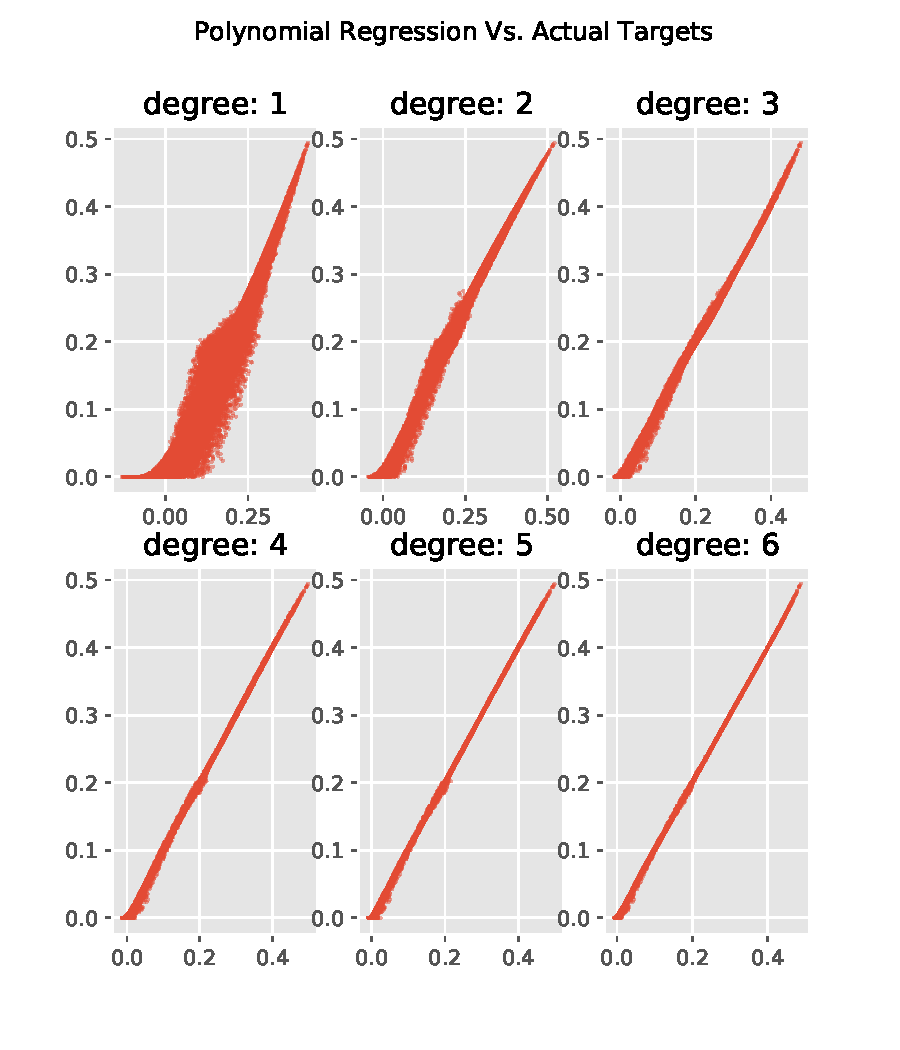
\includegraphics{Figures/polynomialEuroC.png}
\decoRule
\caption[Polynomial Regression Predictions Vs. Actual Prices]{Predicted price based on polynomial regression of varying degree}
\label{fig:PolynomialEuroC}
\end{figure}

\begin{table}[th]
\caption{In-sample validation error for polynomial regression and MLPs on European call option}
\label{tab:euroPerformance}
\centering
\begin{tabular}{l l}
\toprule
\textbf{Model} & \textbf{Valalidation Loss} \\
\midrule
Linear Reg. & 0.000631 \\
2. degree  poly.  & 0.000069 \\
3. degree poly & 0.000013\\
4. degree poly.  & 0.000004 \\
5. degree poly.  & 0.000002 \\
6. degree poly. & 0.000001\\
MLPs        & 0.000003\\
\bottomrule\\
\end{tabular}
\end{table}
Table \ref{tab:euroPerformance} is created to compare the performance for each model. The table confirms that the linear regression has a worse fit than the other models with higher capacity. The difference on the MLPs and best performing polynomial model are less than $1\cdot 10^{-6}$. The difference is almost negligible so the fit for MLPs and polynomial regression of degree 4-6 performs all very well on the in-sample training data in terms of the validation loss.

%-----------------------------------
%	SUBSECTION 3
%-----------------------------------
\subsection{Performance}
The model performance is evaluated by MSE, RMSE, MAE and coefficient of determination, where all the measures evaluate how close the model predictions are with the actual targets. The first three measures ranges are $\mathbb{R}^+$, where the goal is to have the lowest value possible. For MSE close to 0 means that the model predictions does not differ a lot from the observed targets. The RMSE and MAE are same kind of measure, but the deviation is measured slightly different. The coefficient of determination has range $(-\infty, 1]$, where a higher value indicate a better model. Coefficient of determination provides a measure of how well observed targets are predicted by the model, based on the proportion of total variation of targets explained by the model.

\subsubsection{European Call Option}
The European call option is trained with the algorithm and hyperparameters described in the training section (section \ref{Training}). By the hyperparameter investigation we choose a batch size of 64, learning rate $\eta = 0.001$ and a data set of 300K samples. We compare the MLPs regression with the polynomial regression. Table \ref{tab:ComparePolyWithMLPS} shows that the MLPs is superior at extrapolating, because the MLPs performs better on all metrics on the out-of-sample test data sets compared to fitted polynomial regressions with a degree between 1 and 6. For the in-sample test data set the polynomial regression of order 6 and MLPs perform almost equally well, but the polynomial regression of 6. degree is a classical example of overfitting. The in-sample test data is similar to the in-sample training data, hence we expect the same magnitude of error for the test set as for the training set for in-sample testing. The performance measures show that the polynomial regression that was performing well on the in-sample data set was due to overfitting, because the high order polynomial regression does perform poorly on out-of-sample data (table \ref{tab:ComparePolyWithMLPS}). For the 6. order polynomial regression, we see a negative coefficient of determination, which means the model performs worse than the model that predicts the sample mean. This means the 6. degree polynomial have bad performance for out-of-sample data. \\

\begin{table}[th]
\caption{Performance comparison of MLPs and polynomial regression on European call option. Shown the best performing regressions in the linear model and the worst performing in terms of MSE for in-sample and out-of-sample data sets (The full table for polynomial regression is found in appendix table \ref{tab:fullEuroCall})}
\label{tab:ComparePolyWithMLPS}
\centering
\begin{tabular}{l l l l l l l }
\toprule
\textbf{Model} & \textbf{Data set} & \textbf{MSE} & \textbf{RMSE} & \textbf{MAE} & \textbf{Coefficent of Determination} \\
\midrule
MLPs & In-Sample & 0.000000 & 0.000629 & 0.000486 & 0.999961\\
& Out-of-Money & 0.000007 & 0.002644 & 0.001551 & 0.995911\\
& Long Matuiry & 0.000197 & 0.014048 & 0.010061 & 0.986518\\
6. degree poly. & In-Sample & 0.000001 & 0.000958 & 0.000591 & 0.999909\\
1. degree poly. &  & 0.000636 & 0.025212 & 0.018326 & 0.936628\\
2. degree poly. & Long Maturity & 0.001196 & 0.034577 & 0.026287 & 0.918316\\
6. degree poly. &  & 0.043361 & 0.208233 & 0.111190 & -1.962442\\
2. degree poly. & Out-Of-Money & 0.000767 & 0.027694 & 0.022203 & 0.551246\\
1. degree poly. &  & 0.005772 & 0.075973 & 0.060936 & -2.377251\\
\bottomrule\\
\end{tabular}
\end{table}

The MLPs has high predictive strength compared to the polynomials, because it performs well also on out-of-sample data set. The MLPs show that it predicts out-of-money call option with less than a MSE with value $10^{-5}$, where the fit for the long maturity test set has a higher MSE. The European options are liquid in the markets, hence the pricing method can easily be trained on real data. The MLPs fit for in-sample data on the European call option is visualized in figure \ref{fig:MLPsInSampleEuroC}, which shows $\frac{c(S_0,K)}{K}$ predicted from the model and observed target values $\bm{y}$ divided by the strike. The figure shows a overall close fit. For the remaining part of this section the MLPs regression will only be considered, because the polynomial regression has shown bad performance for out-of-sample data.

\begin{figure}[th]
\centering
\includegraphics{Figures/PredictionEuroC.png}
\decoRule
\caption[MLPs Performance on in-sample dataset European Call]{MLPs Performance on in-sample dataset on european call}
\label{fig:MLPsInSampleEuroC}
\end{figure}


\subsubsection{American Put Option}
The American put option is priced with the same MLPs algorithm as for the european call. Table \ref{tab:AmerPerformanceComparision} shows once a again a good fit, hence, we believe, we have a high quality model for the American put option.

\begin{table}[th]
\caption{MLPs Performance on American Put Option}
\label{tab:AmerPerformanceComparision}
\centering
\begin{tabular}{l l l l l l l }
\toprule
\textbf{Data set} & \textbf{MSE} & \textbf{RMSE} & \textbf{MAE} & \textbf{$R^2$} \\
\midrule
In-Sample & 0.000002 & 0.001562 & 0.001278 & 0.999634\\
In-The-Money & 0.000012 & 0.003519 & 0.002290 & 0.995778\\
Longer Maturity & 0.000193 & 0.013894 & 0.009213 & 0.980835\\
\bottomrule\\
\end{tabular}
\end{table}

\subsubsection{American Put On Minimum of Two Assets Option TODO! moneyness}
The American put on minimum of two assets option has almost the double amount of parameters compared to the univariate contingent claims, hence the performance might give slightly higher MSE. Table (TODO: what does the table show and the batchsize chosen) \ref{tab:AmerMinPerformanceComparision} shows a good fit for both in-the-money and longer maturity sample, but the MSE is higher as expected compared to the relative prices for the univariate contingent claims. \\ 

\begin{table}[th]
\caption{Performance of the bivariate American put minimum contingent claim}
\label{tab:AmerMinPerformanceComparision}
\centering
\begin{tabular}{l l l l l l l }
\toprule
\textbf{Data set} & \textbf{MSE} & \textbf{RMSE} & \textbf{MAE} & \textbf{$R^2$} \\
\midrule
In-Sample(TODO! Numbers) & 0.099621 & 0.315644 & 0.001278 & 0.999634\\
In-The-Money & 0.510718 & 0.714646 & 0.542326 & 0.988782\\
Longer Maturity & 3.957424 & 1.989328 & 1.413311 & 0.974056\\
\bottomrule\\
\end{tabular}
\end{table}

The MLPs has shown good performance in terms of our performance measures on all the derivatives considered. Next chapter will compare this MLPs model (henceforth referred to as MLPS II) with the closed form solutions, binomial model, LSM and LSM MLPs (henceforth referred to as MLPS I). All the models in this section considered had good performance on the in-sample dataset except of the too simple models linear regression and 2. degree polynomial regression. To test the predictive strength for the models, we tested the models with out-of-sample data. Specifically we consider longer maturity and not at-the-money options.\\

The MLPs II is not based on a model, it is only trained on the available data. This feature makes the MLPs II pricing method versatile because the MLPs could also be used for actual market data or different models to learn patterns. The fact that the method can be extended to real market data is already shown in \parencite{GasparRaquel20}. This section showed how the MLPs can be trained to pricing derivatives with Black-Scholes theory and also seen that the MLPs is preferred over polynomial regression.









